We begin by describing the set of problems one faces when preparing a dataset for the training process.
This includes determining the hardware requirements, the decision of \textit{where} to preprocess the data, and \textit{when} to preprocess, both of which decisions affect the training throughput in multiple ways.

The preprocessing pipeline can be split into steps which are ran \textit{once} ($S_{\textbf{1}}-S_{\textbf{m}}$), called ``offline'' henceforth, and steps which are performed \textit{every iteration} ($S_{\textbf{m+1}}-S_{\textbf{n}}$), called ``online''.
The set of preprocessing steps depends on the dataset and the model input, but generally, any transformation is a step, like cropping an image or encoding a word.
A preprocessing \textit{strategy} is processing up to (and including) a step offline, and the remainder of the pipeline is executed online. Such a split is accomplished by inserting a \textit{save} step which encodes and writes the data to disk (after $S_\textbf{m}$), and a \textit{load} step that reads that data from disk (before $S_{\textbf{m+1}}$).

%\vspace{-0.22cm}
\begin{figure}[h]
  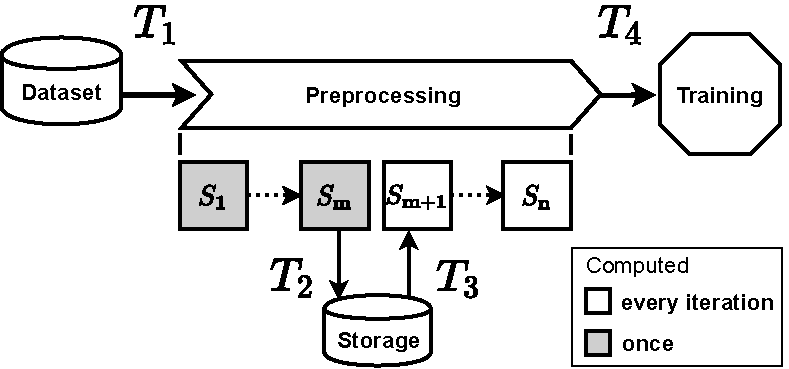
\includegraphics[width=0.4\textwidth]{figures/misc/generic-dl-pipeline-smaller.pdf}
  \vspace{-0.1cm}
  \caption{General DL preprocessing setup with different theoretical throughputs $T_{1}-T_{4}$ between the preprocessing steps $S_{\textbf{1}}-S_\textbf{n}$.}
  \label{fig:generic-dl-pipeline}
\end{figure}
\vspace{-0.2cm}

We conceptually divide the entire DL training process into three parts - the unprocessed dataset, the preprocessing pipeline, and the training (Fig.~\ref{fig:generic-dl-pipeline}).
They are all connected by four theoretical throughputs $(T_{1}-T_{4})$, which can become processing bottlenecks.

\begin{description}[align=left]
\item[$T_1$] is the read throughput from the dataset to the processing units which handle the \textit{offline} preprocessing.
This throughput is determined by hardware capabilities, such as storage devices, interconnects, processing capabilities, and software capabilities, such as file systems or DL frameworks.

\item[$T_2$] is the write throughput from the offline computed preprocessing step(s) ($S_{\textbf{1}}-S_{\textbf{m}}$) to a storage node.
It is dependent on the throughput of each step, the interconnect to the storage node, and its write speed.

\item[$T_3$] is the read throughput from the storage node to the processing units which handle the \textit{online} preprocessing ($S_{\textbf{m+1}}-S_{\textbf{n}}$) and is subject to the same restrictions as $T_1$.

\item[$T_4$] is the final preprocessing throughput when the data is ready to be fed into the training process.
It is restricted by $T_{3}$, the online step(s) performance, and the interconnect to the training process.
As $T_4$ limits the achievable training throughput, it is the most important to optimize.
\end{description}

In practice, it is often impossible to know the actual performance of future DL models or preprocessing pipelines. 
Only partial benchmarks are available to approximate the training throughput of popular DL models~\cite{nvidiabenchmarks2020}.
Even worse, there is no comprehensive throughput analysis of preprocessing pipelines, so one has to estimate the resulting $T_4$ throughput of a pipeline manually for every single deployment to prevent bottlenecks.
Such an estimation is difficult to make, as there are many complexities involved.

One of those is the data encoding after step $S_{\textbf{m}}$, which serializes the entire dataset and places it on a storage device.
The current default way to serialize datasets in two popular DL frameworks is the ``pickle'' encoding for PyTorch~\cite{paszke2019pytorch}, and Protobuf~\cite{protobuf} for TensorFlow~\cite{abadi2016tensorflow}. Both encodings are not optimized for tensor data and may perform poorly. Applying an optimized compression algorithm may be useful but also introduces an additional online decompression step that may affect the $T_4$ throughput.

The deserialization throughput ($T_1$ and $T_3$) depends not only on the encoding but also on the storage solution and its interconnect to the nodes that run the preprocessing pipeline.
A common storage solution in virtualized environments is Ceph~\cite{weil2006ceph}, an object-based storage system.
Such a complex and distributed system's performance depends on the storage hardware and the computing power and must be evaluated on a case-by-case basis.
Without benchmarks for specific hardware setups, it is unclear how to split the pipeline to achieve the maximum throughput~\cite{ra2018understanding,mohan2020analyzing}.

Another variable to consider is the offline preprocessing time, as this may delay the training start.
Long preprocessing times can be prohibitive if not amortized by faster training.

Additionally, some preprocessing steps that feature data augmentation (e.g., random-cropping for images) or shuffling the dataset have to be done online because their results are not deterministic and can not be cached for future epochs.

{\color{diff3}
Some preprocessing steps decrease the dataset size and can make it fit in memory, which would be beneficial over multiple epochs to remove network read effects.
However, preprocessing steps can also be computationally expensive and would better be processed offline which can increase throughput, even if they increase the dataset size.
Both scenarios can benefit the throughput, but it is not obvious to determine without profiling whether caching a dataset or removing a CPU bottleneck is more effective at increasing throughput.
}
%Due to significant bandwith and latency changes from storage to memory, the effects of fitting a dataset into memory can be huge on the throughput.
%However, it is 
%#Increasing dataset sizes make it harder to profile the trade-offs on the entire dataset because this either consumes too much time or induces high costs.
%Sampling could be a possible solution.
%However, it is unknown how many samples have to be processed to yield a reasonable estimate for the entire dataset.

In conclusion, deciding how to split a preprocessing pipeline into offline and online steps is a complex problem.
The importance of the trade-offs may depend on individual scenarios, such as preexisting hardware or framework dependencies, which can not be chosen freely.
To solve this problem and provide guidance and best practices to ML engineers and users, a comprehensive analysis of common DL pipelines is needed that provides a structured overview of the pipelines' performance and insights about the individual steps' trade-offs.
It is also necessary to evaluate whether profiling a small sample of the entire dataset is sufficient to estimate the total processing time, storage consumption, and $T_4$ throughput.
This could reduce profiling overhead.
Finally, a software solution should automate the profiling to quickly generate insights for a specific setup to optimize any given pipeline.

% as executing the steps $S_1 - S_m$ and saving the dataset to the storage device takes time where the pipeline does not produce any throughput. If running a pipeline is time-critical, this can create a trade-off that may or may not be amortized by the number of total iterations and the faster $T_4$ throughput than a slower $T_4$ where every step is computed every iteration.


%What is lacking is a clear methodology of how to analyze, compare and evaluate pipelines.
%Such a methodology should provide 
%A supplementary software solution to generate the findings automatically and provide a programmatical way to pick the most fitting materializtation strategy could reduce costs of DL training processes.

%We exemplifiy the trade-offs for each of the four ML domains with our hardware setup in Section~\ref{sec:evaluation}.

%The following discussion is independent of the model and training process, as we \textit{collect} the training data instead of performing actual training, and this way, evaluate how much $T_4$ throughput we can provide if the data is consumed on the same device. We profiled the different materialization strategies and compare the $T_4$ throughput, the storage consumption and their preprocessing time. The experiments were run with 16 threads. The following results (Figure~\ref{fig:cv-tradeoffs}) were extrapolated with 572~MB of the ILSVRC2012 dataset~\cite{ILSVRC15} (147~GB originally).





 % in an exemplified hardware scenario from our organization. We use OpenStack~\cite{Sefraoui2012} as the cloud OS with KVM-based images~\cite{habib2008virtualization} as virtualization layer to create virtual machines. The VMs can be GPU or CPU VMs, which are connected to a replicated Ceph-based~\cite{weil2006ceph} storage and have local SSD storage. When preprocessing the data on the Ceph storage the interconnect can be a potential bottleneck that restricts the $T_4$ throughput. On the other hand, storing the preprocessed data on a SSD provides less storage capabilies and lower read speeds, which may favor a completely different materialization strategy. Without throughput benchmarks for specific hardware setups and the training pipeline, it is unclear how to split the pipeline in a way that consumes the optimal amount of resources while meeting time requirements.

% One possible instantiation of the DL pipeline with four preprocessing steps from Figure~\ref{fig:generic-dl-pipeline} is to place all of the preprocessing steps on a CPU VM and force a GPU VM to read the fully preprocessed data from the storage node. In this scenario, the interconnect to the GPU VM constitutes a potential read bottleneck which may affect the GPU utilization as it can restrict the throughput $T_4$ of the preprocessing pipeline. Assume another hardware setup, where there is only the GPU VM and the storage node is realized by a local SSD - now $T_4$ is bound by the local file system and the PCIe bus from the GPU\footnote{We look at VMs the same way as hardware nodes for this comparison}~\cite{Fujii2013}. As a single SSD has lower storage capacities or read/write speeds compared to a designated Ceph cluster, this setup may favor a completely different materialization strategy. 



%We showcase the difficulties with job placement and materialization strategies in an exemplified hardware scenario from our organization. We use OpenStack~\cite{Sefraoui2012} as the cloud OS with KVM-based images~\cite{habib2008virtualization} as virtualization layer to create virtual machines to schedule jobs. The VMs can be GPU or CPU VMs, which are connected to a replicated Ceph-based~\cite{weil2006ceph} storage node and realized as 10~Gb SFP+ cables that run over a cluster-grade switch. One of possible instantiations of the DL pipeline with four preprocessing steps from Figure~\ref{fig:generic-dl-pipeline} is to place all of the preprocessing steps on a CPU VM and force a GPU VM to read the fully preprocessed data from the storage node. In this scenario, the interconnect to the GPU VM constitutes a potential read bottleneck which may affect the GPU utilization as it can restrict the throughput $T_4$ of the preprocessing pipeline. Assume another hardware setup, where there is only the GPU VM and the storage node is realized by a local SSD - now $T_4$ is bound by the local file system and the PCIe bus from the GPU\footnote{We look at VMs the same way as hardware nodes for this comparison}~\cite{Fujii2013}. As a single SSD has lower storage capacities or read/write speeds compared to a designated Ceph cluster, this setup may favor a completely different materialization strategy. Without throughput benchmarks for specific hardware setups and the training pipeline, it is unclear how to split the pipeline in a way that consumes the optimal amount of resources while meeting time requirements.


% \begin{description}[align=right,labelwidth=0cm, itemsep=-1.5pt, topsep=0pt]
% \item \texttt{unprocessed}: the raw image files
% \item \texttt{concatenated}: protobuf~\cite{protobuf} encoded files
% \item \texttt{decoded}: RGB images
% \item \texttt{resized}: resized to 256 in $max(\text{height}, \text{width})$
% \item \texttt{full}: pixel centered and randomly cropped to $224\times 224$
% \end{description}

% \begin{figure}
%   \includegraphics[width=0.48\textwidth]{images/misc/training-hardware.pdf}
%   \caption{Hardware instantiation of the DL pipeline from Figure~\ref{fig:generic-dl-pipeline} with the cluster setup in our organization.}
%   \label{fig:training-hardware}
% \end{figure}

%The maximum throughput is achieved with the \texttt{resized} strategy with $4368\;^{MB}/_s$ or $2311\;^{images}/_s$ (Figure~\ref{fig:cv-tradeoffs}). This comes at a cost of a preprocessing time of $46$ minutes and $347$~GB storage consumption, a factor of $2.4\times$ compared to the $147$~GB of the unprocessed dataset. A naive assumption might be that entirely  preprocessing the dataset with the \texttt{full} strategy is the best option to maximize throughput, but it is actually the worst on all counts compared to the other strategies. The reason for that is that the pixel centering from step $S_4$ changes the encoding from \texttt{int8} to \texttt{float32} and in turn increases the storage consumption from $347$~GB to $1389$~GB. This builds up the I/O load on the storage interconnect, which limits the throughput in this hardware setup to $936\;^{MB}/_s$. The \texttt{decoded} strategy shows a similar pattern as it also increases the dataset size to almost $849$~GB and has a throughput of $1217\;^{MB}/_s$, only reaching $28$\% of the \texttt{resized} strategies performance. The next steps would be to profile the actual DL model's throughput and see if a strategy exists that does not constitute a bottleneck and has satisfactory trade-offs in terms of hardware costs and run-time.

%There is no easy solution for the materialization problem as there are always trade-offs to be considered, such as preexisting hardware or framework dependencies which can not be chosen freely.

